\section{Introduction}
\label{sec:intro}

With the rapid proliferation of social media, images are increasingly used as a medium for users to share daily experiences, emotions, and personal viewpoints. 
Visual intention recognition aims to infer the latent purpose conveyed by an image, and has become an important problem in human-centered multimedia analysis \cite{jia_intentonomy_2021, wen_dip_2023}. 
% Unlike explicit textual statements, such visual expressions often imply intentions in an indirect and abstract manner. 
Accurately recognizing these intentions is valuable for a variety of downstream applications, including user interest understanding, psychological and behavioral profiling, broader social media content analysis, \textit{etc}.

Compared with conventional image classification, visual intention recognition is fundamentally more challenging.
In traditional classification tasks, the goal is to assign images to relatively objective semantic categories, such as objects, scenes, or actions. 
In contrast, intention recognition requires mapping visual evidence to abstract and subjective intent labels.
These labels are rarely determined by local visual cues alone; instead, they often emerge from a holistic interpretation of scene context, human activities, object configurations, social interactions, and commonsense knowledge.
Therefore, the main difficulty of this task lies not merely in visual representation learning, but in establishing a reliable bridge between concrete image content and abstract intention semantics.

A central challenge of this task is its inherent ambiguity, which manifests in two distinct forms, as shown in Figure~\ref{fig:teaser} (a).
The first is semantic ambiguity. 
Intent labels are often semantically adjacent, partially overlapping, or hierarchically correlated. 
Different labels may correspond to visually similar patterns, while the same intent may be expressed through diverse appearances. 
This leads to high inter-class similarity and substantial intra-class variation, making fine-grained discrimination particularly difficult.
The second is supervisory ambiguity. 
Since intention recognition is intrinsically subjective, different audiences may infer different yet plausible intentions from the same image. 
As a result, the supervisory signal itself may become unstable, especially for difficult samples with severe disagreement. 
Under such circumstances, directly optimizing against hard labels can force the model to fit oversimplified or unreliable targets, thereby harming the robustness of the learned decision boundaries.

\begin{figure}[t]
\centering
\begin{subfigure}[t]{0.51\linewidth}
\centering
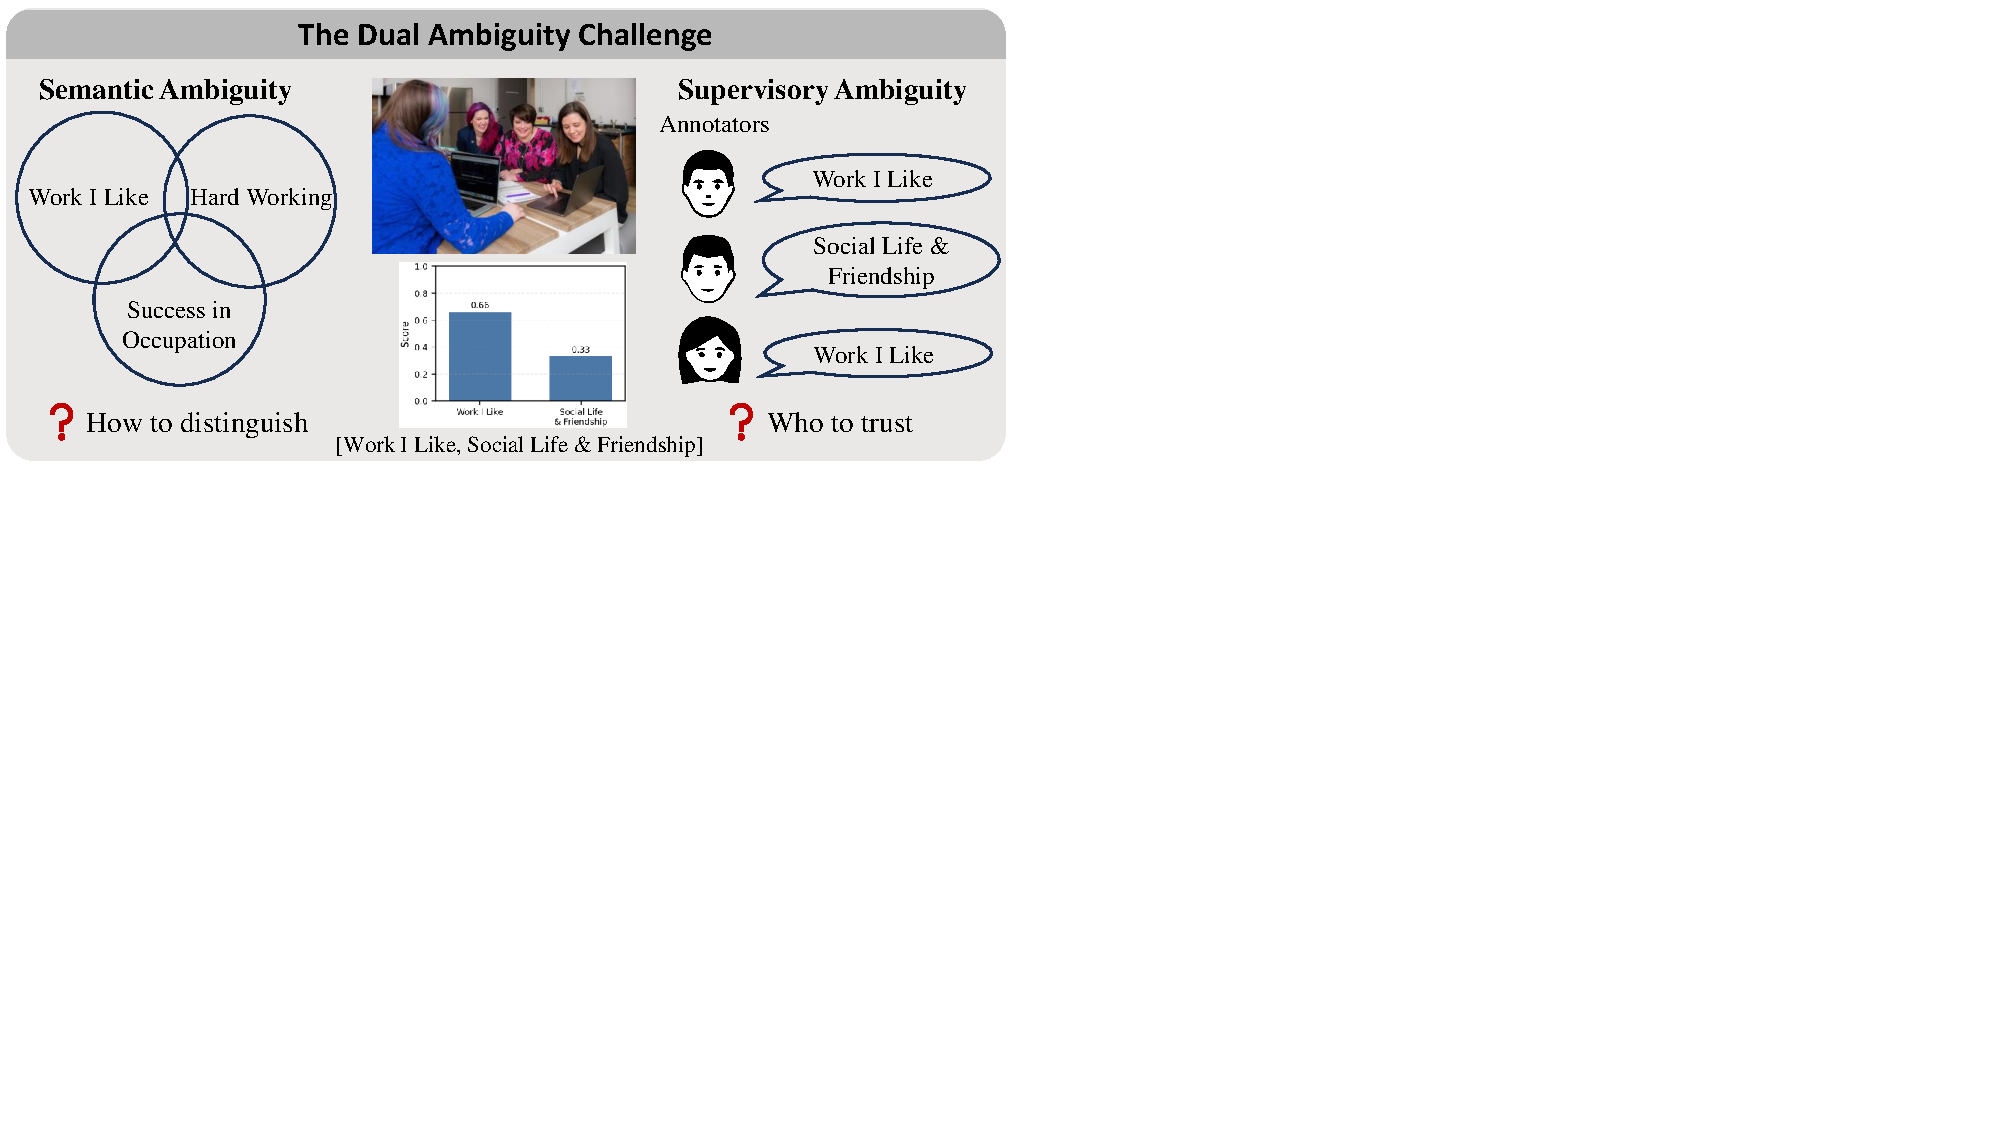
\includegraphics[width=\linewidth]{srcs/teaser_a.pdf}
\end{subfigure}
\hfill
\begin{subfigure}[t]{0.43\linewidth}
\centering
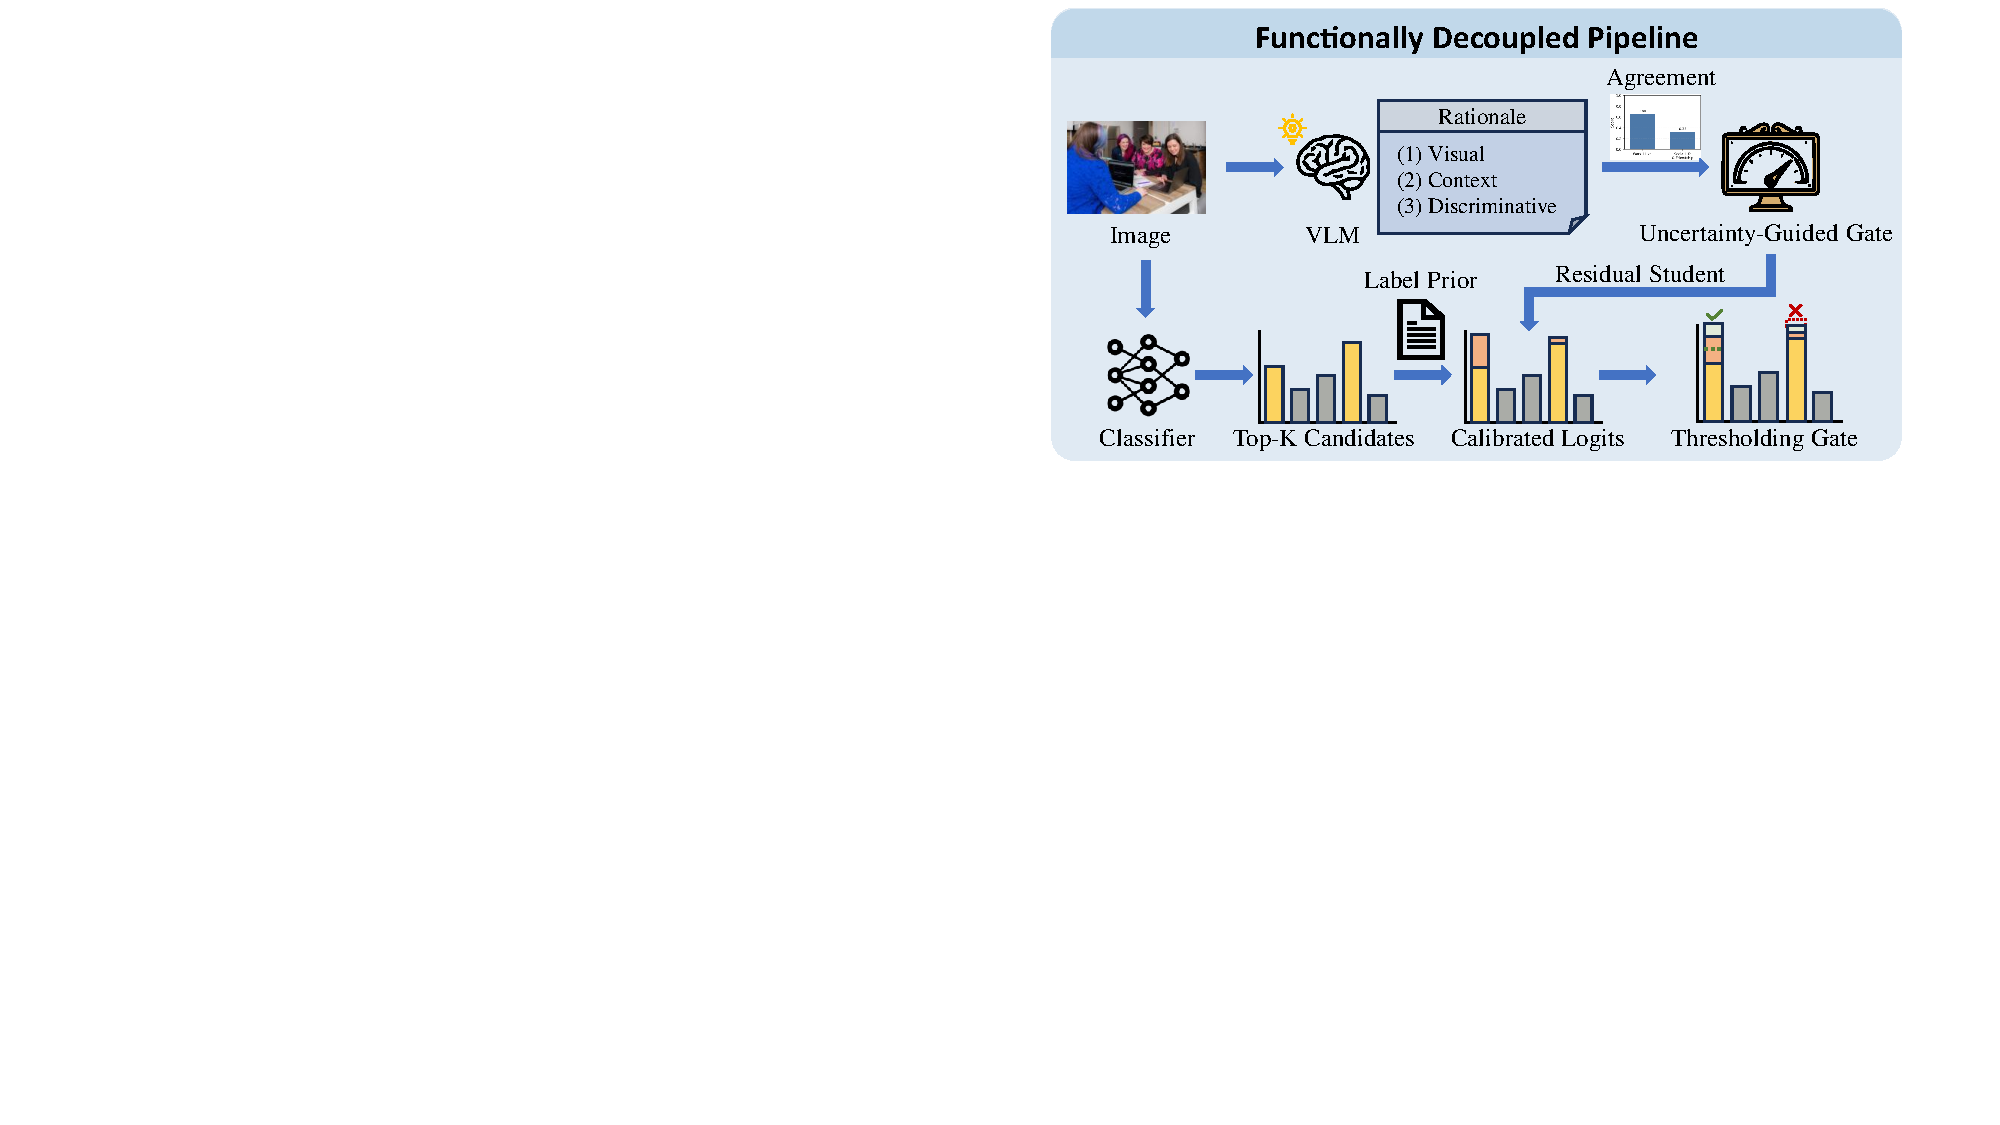
\includegraphics[width=\linewidth]{srcs/teaser_b.pdf}
\end{subfigure}
\caption{\textbf{Functionally decoupled ambiguity modeling in FDIL.} \textbf{(a) The dual ambiguity challenge:} subjective visual intent recognition is fundamentally bottlenecked by \textit{semantic ambiguity} (highly overlapping conceptual boundaries) and \textit{supervisory ambiguity} (annotator disagreement and unstable training targets). \textbf{(b) Functionally decoupled pipeline:} FDIL separates ambiguity-aware semantic refinement from ambiguity-aware semantic supervision. Semantic Local Reranking and Calibration (SLR-C) builds a semantic prior from textual cues to provide structured candidate semantics, while Uncertainty-guided Text Distillation (UTD) stabilizes learning under disagreement through rationale-guided text distillation and supports image-aware prediction on top of the semantic prior.}
\label{fig:teaser}
\end{figure}

Existing studies have attempted to alleviate these difficulties from different perspectives. 
Prototype-based methods, \textit{e.g.} PIP-Net \cite{wang_prototype-based_2023}, introduce representative anchors to reduce feature-space confusion. 
Structure-aware methods, including CPAD \cite{ye_cross-modality_2023} and HLEG \cite{shi_learnable_2023}, exploit hierarchical label relationships to enhance multi-level semantic modeling and strengthen supervision. 
From the perspective of label quality, LabCR \cite{shi_label-aware_2024} explicitly models label shifting and label blemish to better cope with imperfect annotation distributions. 
More recently, knowledge-enhanced approaches have recognized that visual evidence alone is often insufficient for subjective intention understanding. 
IntCLIP \cite{leonardis_synergy_2025} incorporates the vision-language alignment knowledge of CLIP into the task, while IntentMLM \cite{wang_unlocking_2026} further leverages multimodal large models, caption generation, and retrieval to perform more holistic intention perception.

Although these methods have yielded encouraging progress, they typically treat one perspective of ambiguity as dominant. 
In our view, the core difficulty of subjective visual intention recognition is not any single ambiguity alone, but the coexistence of supervisory ambiguity and semantic ambiguity, which interfere with different functional components of the system. 
The former primarily corrupts supervision by compressing diverse subjective interpretations into rigid targets, whereas the latter primarily distorts local decision geometry by making neighboring labels difficult to separate. 
Treating these two failure modes within one mechanism may therefore be suboptimal, as it is difficult to simultaneously achieve robust learning on disagreement-prone samples and precise discrimination among closely related intents.

Motivated by this observation, we propose the \textbf{FDIL} (\textbf{F}unctionally \textbf{D}ecoupled \textbf{I}ntent \textbf{L}earning), a functionally decoupled framework for subjective intent recognition, as illustrated in Figure~\ref{fig:teaser}(b), where fixed semantic priors provide structured candidate semantics, uncertainty-aware text teachers stabilize ambiguous supervision, and a residual student learns image-aware intent prediction on top of the semantic prior.
We decouple ambiguity handling into two complementary functions.
First, Semantic Local Reranking and Calibration (SLR-C) provides ambiguity-aware semantic refinement: heterogeneous lexical, canonical, and scenario priors define a semantic prior that supplies structured candidate semantics.
Second, Uncertainty-guided Text Distillation (UTD) provides ambiguity-aware semantic supervision: a text-only teacher distilled from rationale embeddings regularizes the visual model according to annotator agreement, improving robustness under subjective supervision and supporting image-aware prediction on top of the semantic prior.
Together, these two functions improve both robustness and discriminability without introducing high architectural complexity.

Extensive experiments on the Intentonomy dataset show that our FDIL consistently outperforms strong existing baselines and recent state-of-the-art methods, yielding improvements in both hard-sample robustness and overall multi-label prediction quality.

The main contributions of this work are summarized as follows:
\begin{itemize}
    \item We reformulate visual intention recognition as a \emph{functionally decoupled} ambiguity problem, and show that supervisory ambiguity and semantic ambiguity should be handled by different functional modules rather than by one unified mechanism.
    \item We propose Semantic Local Reranking and Calibration (SLR-C) together with residual semantic refinement, where heterogeneous textual priors first define a semantic prior with structured candidate semantics and a lightweight residual student further adapts prediction to image evidence.
    \item We propose Uncertainty-guided Text Distillation (UTD), which leverages annotator disagreement as an uncertainty signal to adaptively introduce semantic guidance, improving robustness under ambiguous supervision.
\end{itemize}

